\documentclass{article}
\usepackage[utf8]{inputenc}
\usepackage{parskip}
\usepackage{graphicx}
% image path
\graphicspath{{./images/}}


\title{Documento di specifica software per il progetto di Ingegneria del Software Avanzata\par
    \textit{Progetto:} \textbf{ISA Blog}\\}

\author{Jipwouo chiege planck anders}
\date{}

\begin{document}

\maketitle
\clearpage

\tableofcontents
\clearpage

\section{Introduzione}
\label{sec:introduzione}

In questo documento si riportano le specifiche software di un servizio web ISA Blog.

\section{Requisiti}
\label{sec:requisiti}

\subsection{ISA Blog}

In primis, \textbf{ISA blog} è una piattaforma di blogging open-source, costruita con tecnologie moderne
dove gli utenti possono condividere i propri pensieri e interagire con gli altri utenti.\\

\begin{itemize}
    \item Di ogni utente, l'applicazione deve memorizzare tramite il processo di registrazione:
    \begin{itemize}
        \item il \textbf{nome utente}
        \item l'\textbf{immagine} del profilo
        \item l'\textbf{indirizzo email}
        \item il \textbf{provider} (Google, GitHub, email)
        \item il \textbf{token} di autenticazione
        \item la \textbf{data} e l'\textbf{ora} di creazione
        \item la \textbf{data} e l'\textbf{ora} di ultima modifica
    \end{itemize}
    \item Di ogni articolo, l'applicazione deve memorizzare:
    \begin{itemize}
        \item il \textbf{titolo}
        \item il \textbf{contenuto}
        \item la \textbf{data} e l'\textbf{ora} di creazione
        \item l'\textbf{autore} (nome utente, immagine profilo, ecc.)
        \item il \textbf{numero di like}
        \item il \textbf{i commenti}
        \item il \textbf{numero di bookmark}
        \item la \textbf{categoria} (es. informatica, matematica, fisica, ecc.)
        \item l'\textbf{immagine} di copertina
        \item l'\textbf{immagine} del post
    \end{itemize}
    \item ogni articolo può avere uno o più commenti e l'applicazione deve memorizzare:
    \begin{itemize}
        \item il \textbf{contenuto} del commento
        \item la \textbf{data} e l'\textbf{ora} di creazione
        \item l'\textbf{autore} (nome utente, immagine profilo, ecc.)
        \item il articolo a cui si riferisce
    \end{itemize}
    \item ogni like è associato ad un articolo e all'utente che ha messo il like.\\
    \item ogni bookmark è associato ad un articolo e all'utente che ha messo il bookmark.
\end{itemize}


\subsection{Isa Blog API base on Supabase}

Supabase fornisce un'interfaccia RESTful per accedere ai dati del database.
L'applicazione deve chiedere a supabase di restituire i dati in formato JSON per le seguenti query:

\begin{itemize}
    \item profile (utente):
    \begin{itemize}
        \item in base all'ID dell'utente (GET)
        \item in base all'ID dell'utente (PUT)
        \item in base all'ID dell'utente (DELETE)
    \end{itemize}
    \item articoli:
    \begin{itemize}
        \item la lista di tutti gli articoli (GET) con i relativi commenti, like e bookmark associati ad anche il profilo dell'autore associato
        \item in base all'ID del articolo (GET) con i relativi commenti, like e bookmark associati ad anche il profilo dell'autore associato
        \item in base ai dati del articolo (articolo) (titolo, contenuto, categoria, immagine di copertina, immagine del articolo)
    \end{itemize}
    \item comments:
    \begin{itemize}
        \item la lista di tutti i commenti (GET) con il profilo dell'autore associato
        \item in base ai dati del commento (articolo) (contenuto, articolo a cui si riferisce)
    \end{itemize}
    \item likes:
    \begin{itemize}
        \item un base all'ID del articolo (GET) con il profilo dell'autore associato al like
        \item toggle like (POST) in base all'ID del articolo (like/unlike)
    \end{itemize}
    \item bookmarks:
    \begin{itemize}
        \item un base all'ID del articolo (GET) con il profilo dell'autore associato al bookmark
        \item toggle bookmark (articolo) in base all'ID del articolo (bookmark/unbookmark)
    \end{itemize}
    \item Per ogni query $s$ ad nostro server db, il server deve rispondere con uno dei seguenti codici di stato HTTP:
    \begin{itemize}
        \item \textbf{200 OK} se la query è andata a buon fine
        \item \textbf{400 Bad Request} se la query non è corretta
        \item \textbf{401 Unauthorized} se l'utente non è autenticato
        \item \textbf{403 Forbidden} se l'utente non ha i permessi per eseguire la query
        \item \textbf{404 Not Found} se la risorsa richiesta non esiste
        \item \textbf{500 Internal Server Error} se c'è un errore interno al server
    \end{itemize}
    \item Ogni query $s$ è protetta da un token di autenticazione che deve essere inviato come header HTTP.
    \item Per quanto riguarda l'interfaccia web, essa deve permettere di visualizzare la lista degli articoli, in particolare:
    \begin{itemize}
        \item il titolo del articolo (con un link al articolo)
        \item l'immagine di copertina del articolo
        \item il numero di like
        \item il numero di commenti
        \item il numero di bookmark
        \item la categoria del articolo
        \item l'autore del articolo
        \item la data di creazione del articolo
        \item il overview del contenuto del articolo
        \item bottoni per mettere like, commentare e bookmark
    \end{itemize}
    \item L'etichetta dello stato dell'icona like, commento e bookmark deve essere:
    \begin{itemize}
        \item sempre \textbf{blue} per l'icona del commento (sempre attiva) numero di commenti.
        \item \textbf{giallo} se il articolo è stato salvato dall'utente registrato
        \item \textbf{rosso} se il articolo è stato likato da l'utente registrato
    \end{itemize}
    \item L'applicazione deve offrire inoltre delle REST API per poter ottenere:
    \begin{itemize}
        \item la lista degli endpoint nel sistema con il loro stato
        \item la lista degli endpoint attivi
        \item un endpoint specifico con il suo stato (conoscendone l'URL)
    \end{itemize}
\end{itemize}

\subsection{User management}

Per utilizzare l'applicazione e visualizzare lo stato degli endpoint è necessario disporre di un account utente.
L'interfaccia web deve permettere di registrarsi, di effettuare il login e di effettuare il logout.

Per ogni utente, l'applicazione deve memorizzare:
\begin{itemize}
    \item il \textbf{nome utente}
    \item l'\textbf{immagine} del profilo
    \item l'\textbf{indirizzo email}
    \item il \textbf{provider} (Google, GitHub, email)
    \item il \textbf{numero di telefono}
    \item il \textbf{mestiere} (default: viewer)
\end{itemize}

Un utente registrato sulla piattaforma può aggiungere nuovi articoli e interagire con gli articoli esistenti.

\clearpage
\section{Data flow diagram}
\label{sec:data_flow_diagram}


\begin{figure}[h]
    \centering
    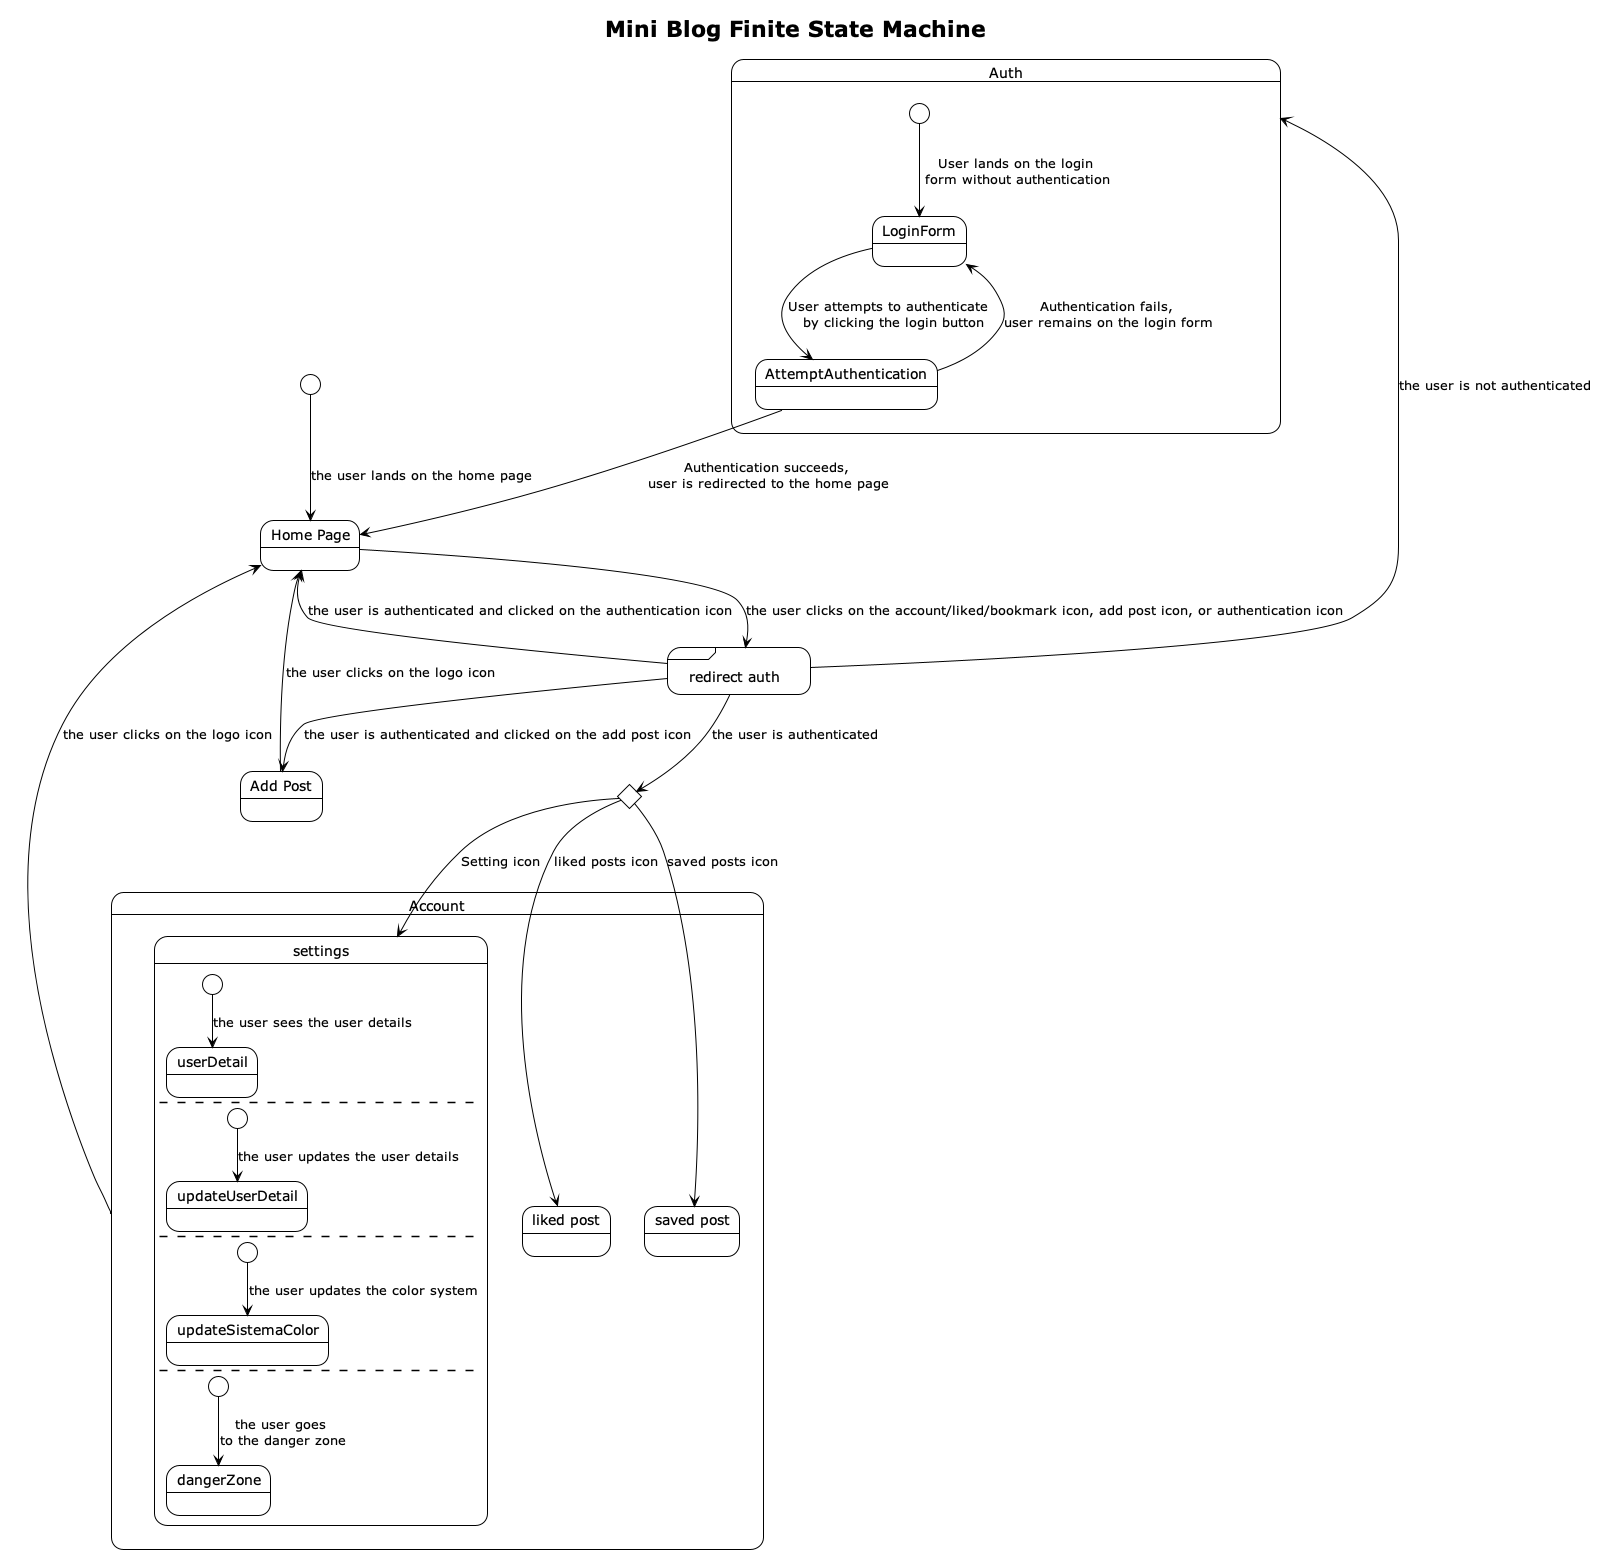
\includegraphics[width=1.3\textwidth]{ingblog_flow}
    \caption{ISA Blog flow}
    \label{fig:figure5}
\end{figure}

%raffinameto di administration
\begin{figure}[h]
    \lefting
    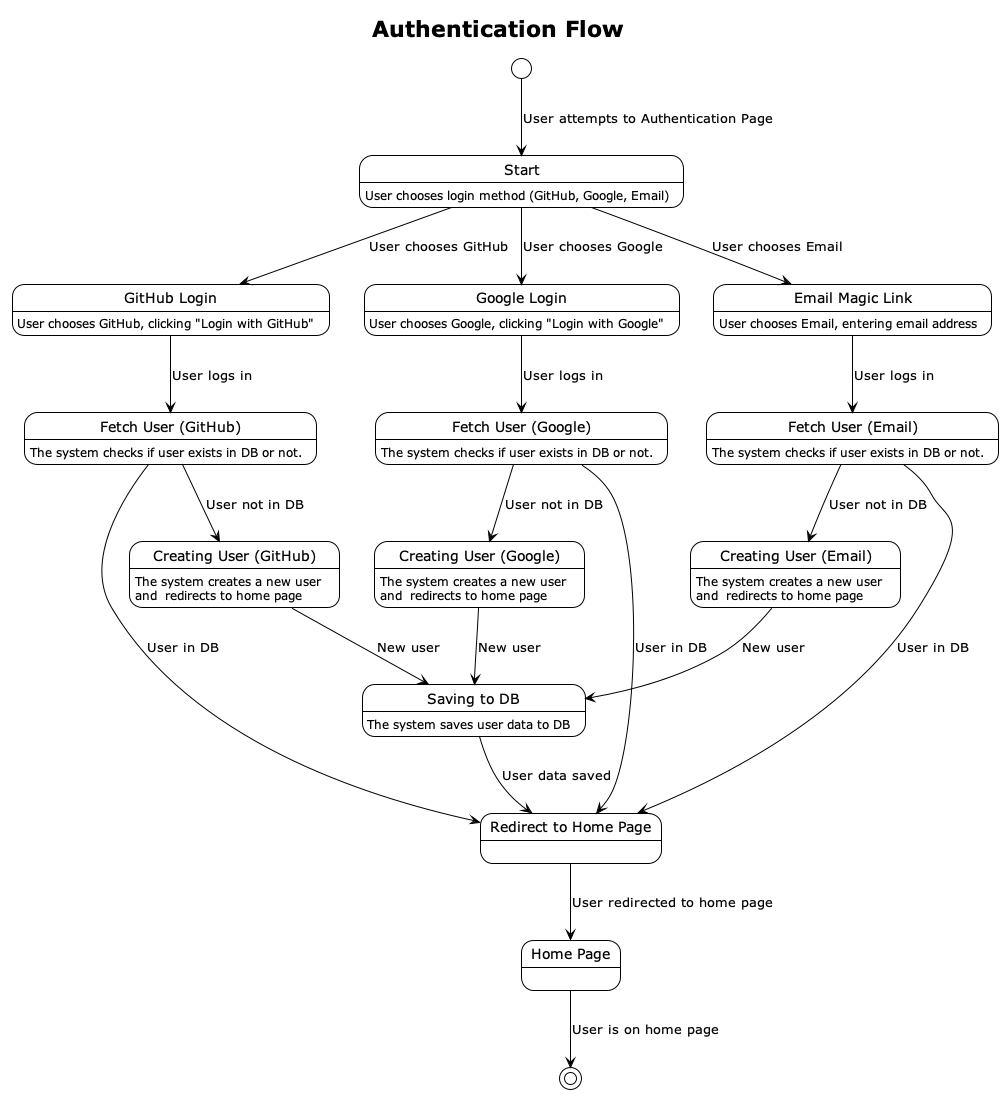
\includegraphics[width=1.3\textwidth]{authentication_flow}
    \caption{autenticazione flow}
    \label{fig:figure4}
\end{figure}

\begin{figure}[h]
    \lefting
    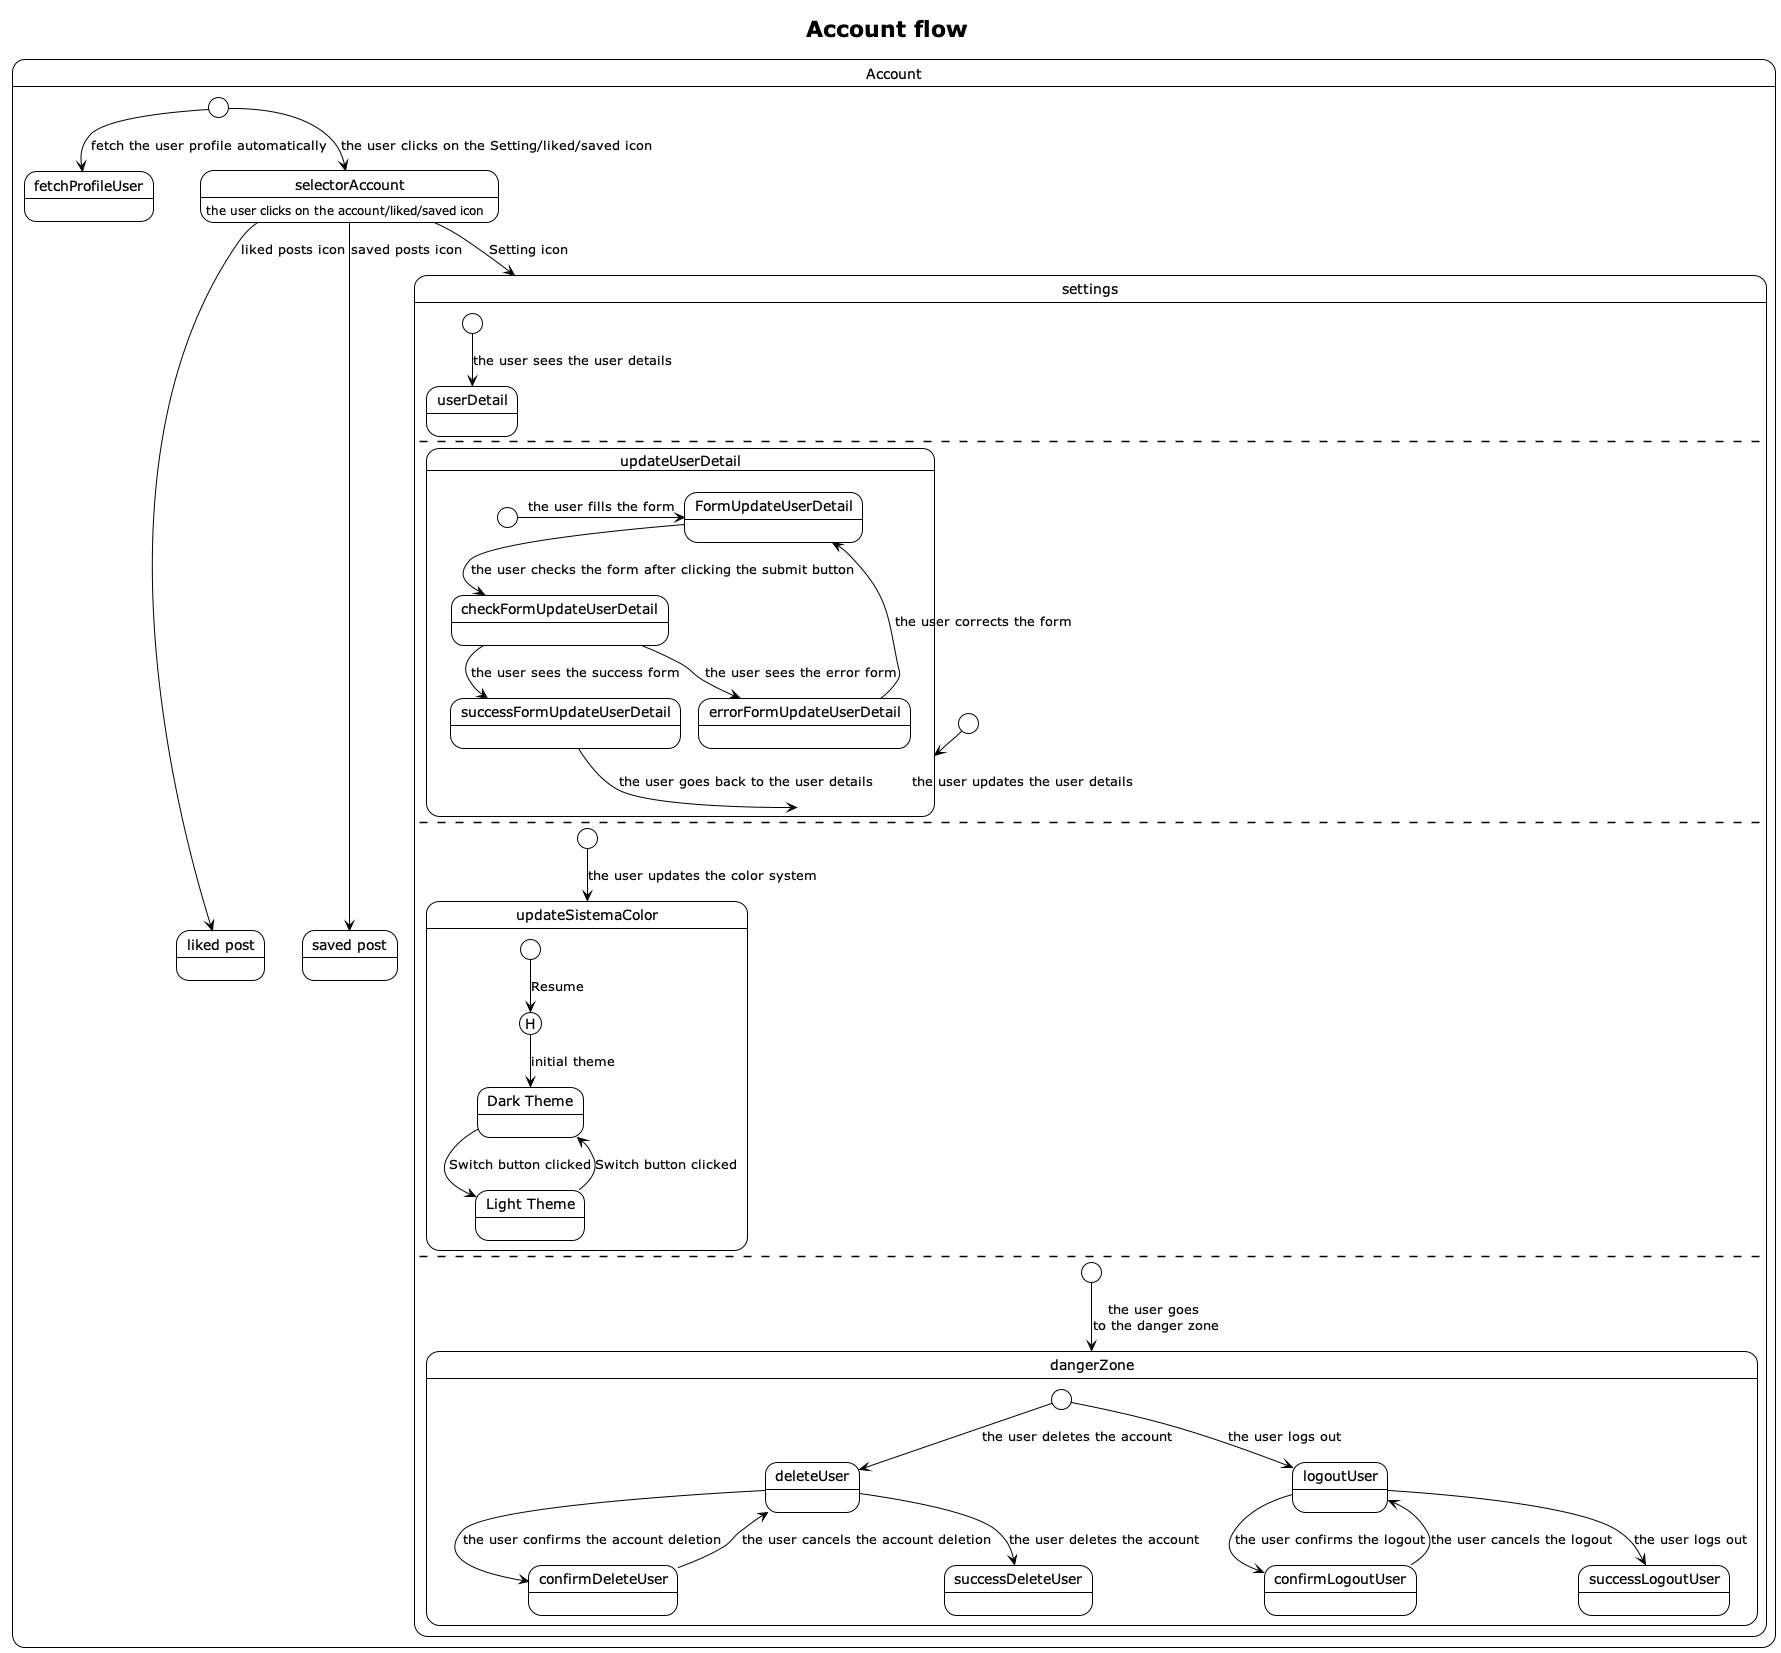
\includegraphics[width=1.3\textwidth]{account_page_flow}
    \caption{Account page flow}
\end{figure}

%raffinameto di sparql endpoint status reporting
\begin{figure}[h]
    \lefting
    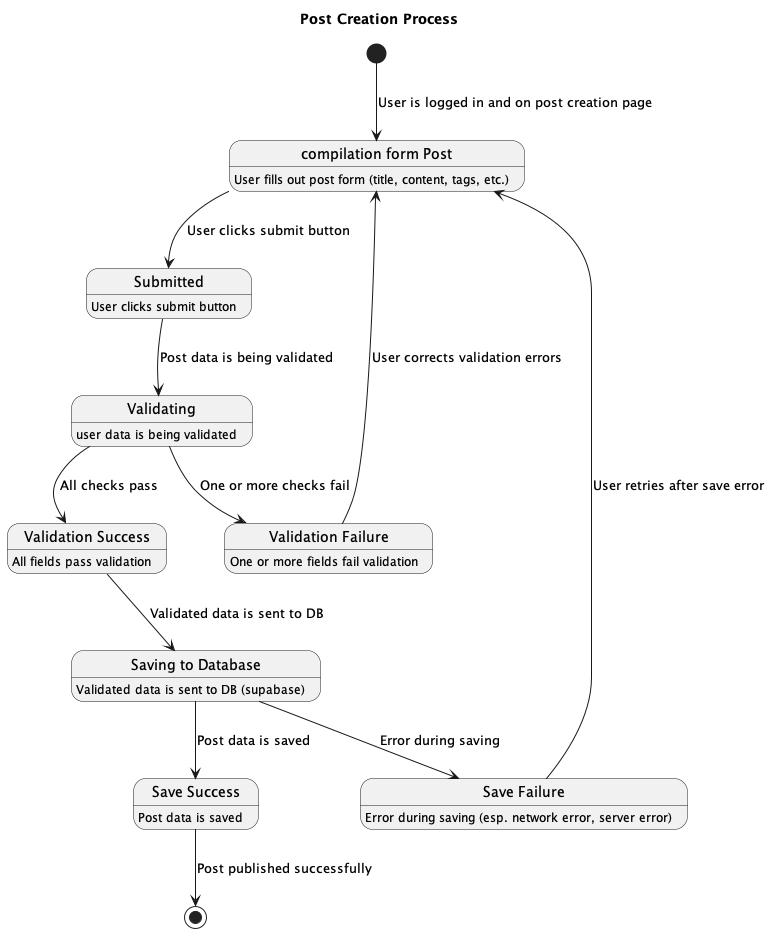
\includegraphics[width=1.3\textwidth]{creazione_post_flow}
    \caption{creazione post}
    \label{fig:figure3}
\end{figure}

\begin{figure}[h]
    \lefting
    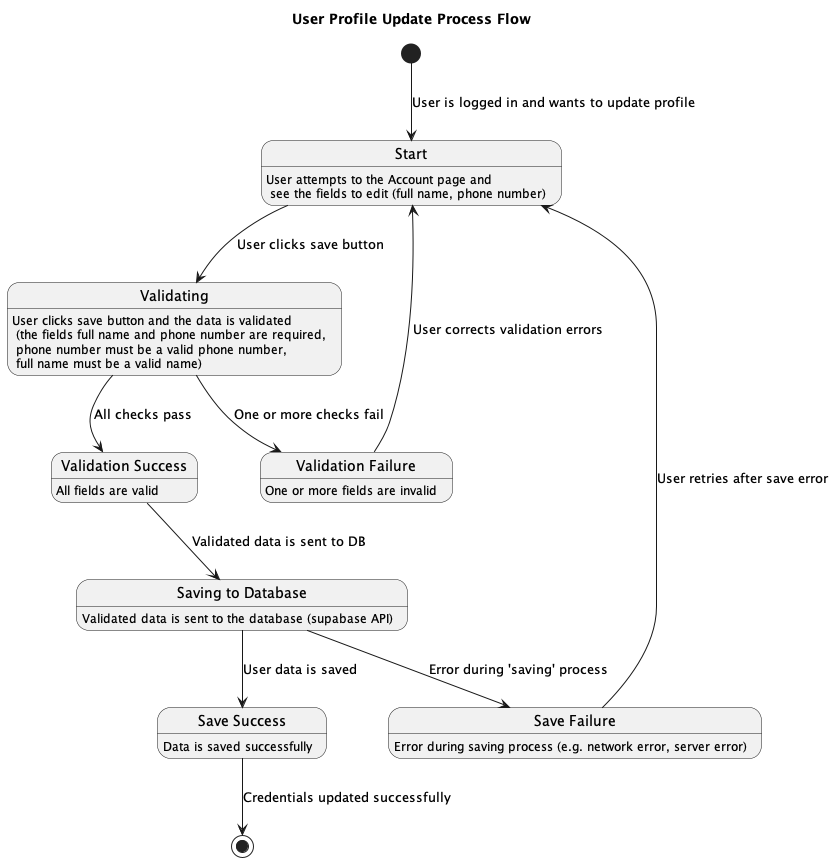
\includegraphics[width=1.3\textwidth]{modifica_profilo_flow}
    \caption{modifica profilo}
    \label{fig:figure2}
\end{figure}

\begin{figure}[h]
    \lefting
    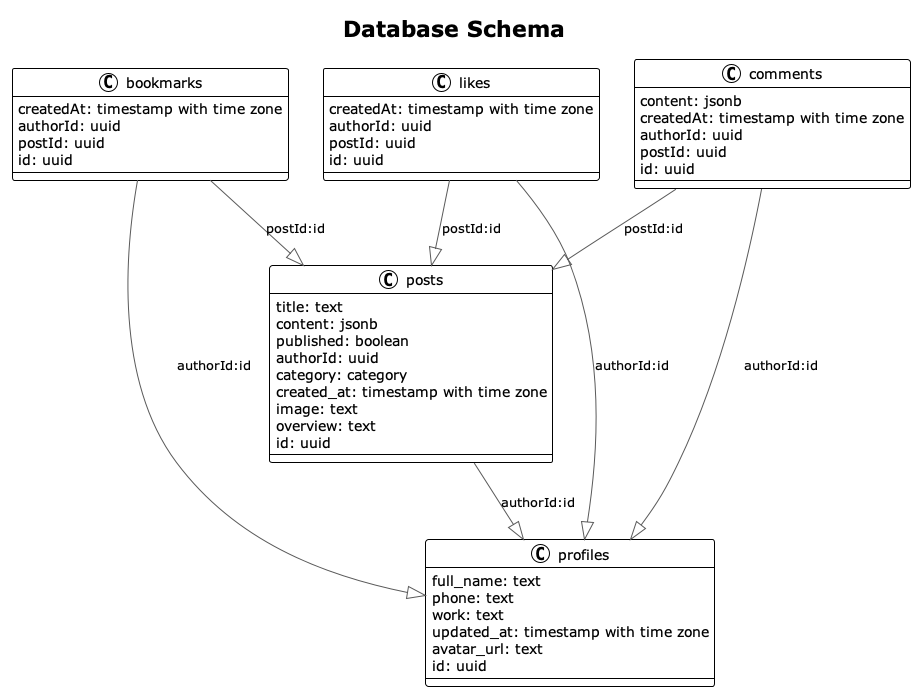
\includegraphics[width=1.3\textwidth]{database}
    \caption{database rapresentazione}
    \label{fig:figure}
\end{figure}

\end{document}


